\documentclass[12pt]{jarticle}
\usepackage[dvipdfmx]{graphicx}
\usepackage[dvipdfmx]{color}
\usepackage{braket}
\usepackage{here}
\usepackage{amsmath}
\usepackage{amssymb}
\usepackage{physics}
\title{原子核の変形と中性子ドリップラインに対するクーロン相互作用の効果}
\author{萩原健太}
\date{2023年1月21日}
\begin{document}

\begin{center}
    {\Large
        原子核の変形と中性子ドリップラインに対するクーロン相互作用の効果
    }
\end{center}
\vspace{1em}
\begin{flushright}
  201910867 萩原健太

  指導教員:中務孝
\end{flushright}


\section{背景}
\subsection{原子核の性質}
%http://ne.phys.kyushu-u.ac.jp/ne.phys.kyushu-u.ac.jp/wakasa/public_html/np17/np6.pdf
%https://www.jicfus.jp/jp/2017-01/#:~:text=%E5%AE%89%E5%AE%9A%E3%81%AA%E5%8E%9F%E5%AD%90%E6%A0%B8%E3%81%AB%E3%81%AF,%E3%81%93%E3%81%A8%E3%81%A7%E3%81%99%EF%BC%88%E5%9B%B31%EF%BC%89%E3%80%82
原子核は正の電荷をもつ陽子と電荷をもたない中性子から構成され、それぞれをまとめて核子と呼ぶ。
核子同士には短距離力の核力が作用しており、クーロン相互作用による斥力に逆らって核子同士を結合させている。
核子の数に着目して、核子数$A$が同じ原子核を同重体 (isobar)、陽子数Zが同じ核種を同位体 (isotope)、中性子数Nが同じ原子核を同調体 (isotone)のような言葉が用いられる。

%結合エネルギーの飽和性の話
原子核は量子多体系であり、各核子の静止エネルギーから原子核の静止エネルギーを引いたものを結合エネルギーとして定義できる。
\[
    E_B (N,Z) = [Nm_n + Zm_p - M(N,Z)]c^2
\]
ここで$E_B (N,Z)$が結合エネルギー、$N$が中性子数、$Z$が陽子数である。
$m_n$、$m_p$、および$M(N,Z)$はそれぞれ中性子と陽子、原子核の静止質量を表す。
$A$が20程度の小さな核では$E_B$は核子数$A$とともに急激に大きくなるが、それを超えるとほぼ$A$に比例する。
つまり核子数当たりの結合エネルギーはほとんど一定になる性質があり、これを結合エネルギーの飽和性と呼ぶ。
同重体の中で結合エネルギーが最も大きく安定な原子核は、比較的軽い核では$N=Z$の核であるが、
一般に重い核になると陽子間に働くクーロン斥力の効果により$N>Z$になる傾向がある。
\begin{figure}[H]
    \centering
    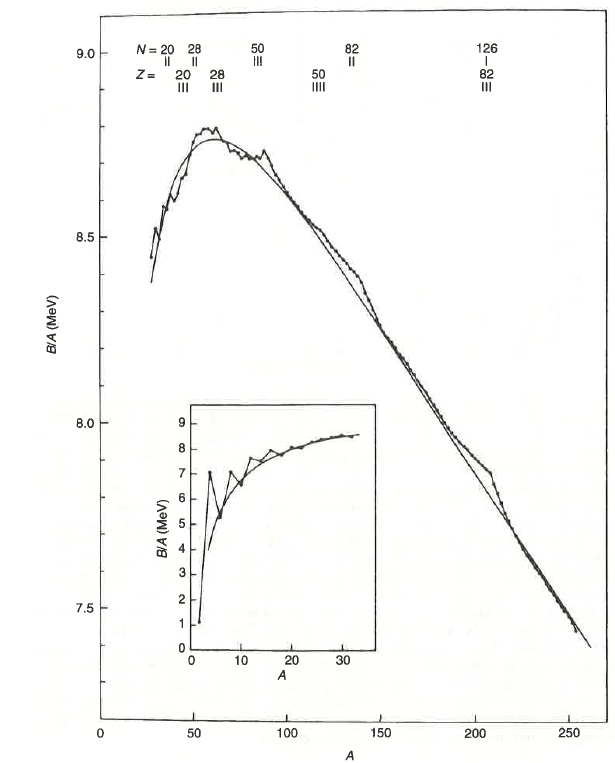
\includegraphics[width=100mm]{../bindingE.png}
    \caption{
        β安定線内に存在する原子核の核子当たりの結合エネルギー。文献\cite{NuclearStructure}Fig. 3.8から引用
    }\label{fig:bindingE}
\end{figure}
図\ref{fig:bindingE}に示すように核子当たりの結合エネルギーはある程度滑らかな関数であるがところどころ特に大きくなり、周りの原子核に比べて特別に安定するような核が存在する。
これは次の$N$および$Z$の原子核で見られる性質であり、このような$N$と$Z$を魔法数という。
\[
    N,Z = 2,8,20,28,50,82,126,…
\]
例えば酸素16のように$N$と$Z$がともに魔法数であるような原子核は二重閉殻と呼ばれ特に安定して存在する。

%密度の飽和性の話
α粒子、核子、電子などの散乱実験から原子核の大きさを調べることが出来る。
電子散乱などから荷電分布を測ることに成功しており、原子核の半径は質量数の1/3乗に比例することが判明している。
\[
    R_B = r_0 A^{1/3} 
\]
半径から出発することで原子核の体積$V$や、単位体積当たりの核子の数:平均核子密度$\braket{\rho}$などの物理量を考えることが出来る。
\begin{equation}
    \ev*{\rho} = \frac{A}{V} = \frac{A}{r_0^{3}A}
\end{equation}
このように単位体積当たりに含まれる核子の数は質量数に依存しないことが分かっている。
この性質を密度の飽和性と呼ぶ。

%ドリップライン
陽子数に対して中性子数が多くなると中性子の結合エネルギーは小さくなり、やがて0になる。
核図表上でこの核種を結んだ線を中性子ドリップラインと呼び、中性子過剰側の存在限界を表す。
逆に陽子数を増やしていくと陽子の結合エネルギーが小さくなり、中性子の場合と同様にやがて0になる。
このような核種を結んだ線は陽子ドリップラインと呼ばれ、陽子過剰側の存在限界を表す。
陽子過剰の場合にはクーロン相互作用による斥力で不安定化しやすくなるため、陽子過剰側に比べて中性子過剰側に存在する原子核の方が多くなる。
陽子過剰側もしくは中性子過剰側にはどれほどの原子核が存在するのか、という問いに対して多くの議論が進められている。
ドリップラインの研究は宇宙での元素合成メカニズムなどにもつながり、学際的な関心も高い分野である。

%\subsection{原子核の変形に関する実験的報告}
%変形についての論文参照
%準備中
%
\subsection{変形}
原子核の形に着目すると、陽子数や中性子数が魔法数に近い場合は球形に近く、魔法数から離れた場合には変形して存在することが実験と理論の両面から確認されている。
多くの原子核はパリティ対称性と軸対称性を破らない変形を持つと考えられており、対称軸に対して細長く伸びたような変形をするプロレート型変形と、潰れたようなオブレート型変形の2種類に分けられる。
図\ref{fig:deformation}には一般的な変形を表示したが、上記の変形の他にもパリティ対称性や軸対称性を破るような変形も予想されており、原子核の研究の大きなテーマの一つである。
\begin{figure}[H]
    \centering
    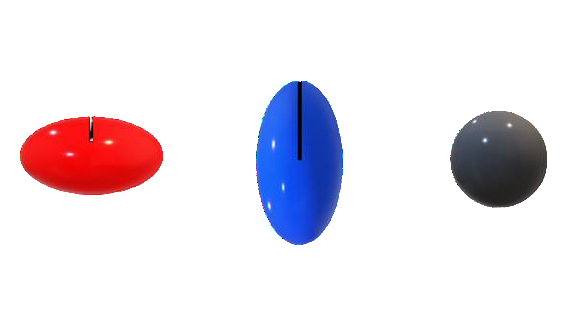
\includegraphics[width=100mm]{../変形図.png}
    \caption{
        原子核の変形の一例。
        本研究で扱う四重極変形の場合は、以下で定義する変形度$\beta$の符号によって回転軸に並行に伸びたプロレート型変形、潰れたようなオブレート型に大別される。
        }\label{fig:deformation}
\end{figure}
四重極変形についての研究も盛んで、\cite{ebata}では$Z=6-92$の元素のうち$N=Z$と$N=2Z$の領域にある
偶偶核の変形度について調査が行われており、プロレート型変形をする原子核が最も多いことが報告されている。
論文内の結果を図\ref{fig:deformation_ebata-san}に掲載する。
\begin{figure}[H]
    \centering
    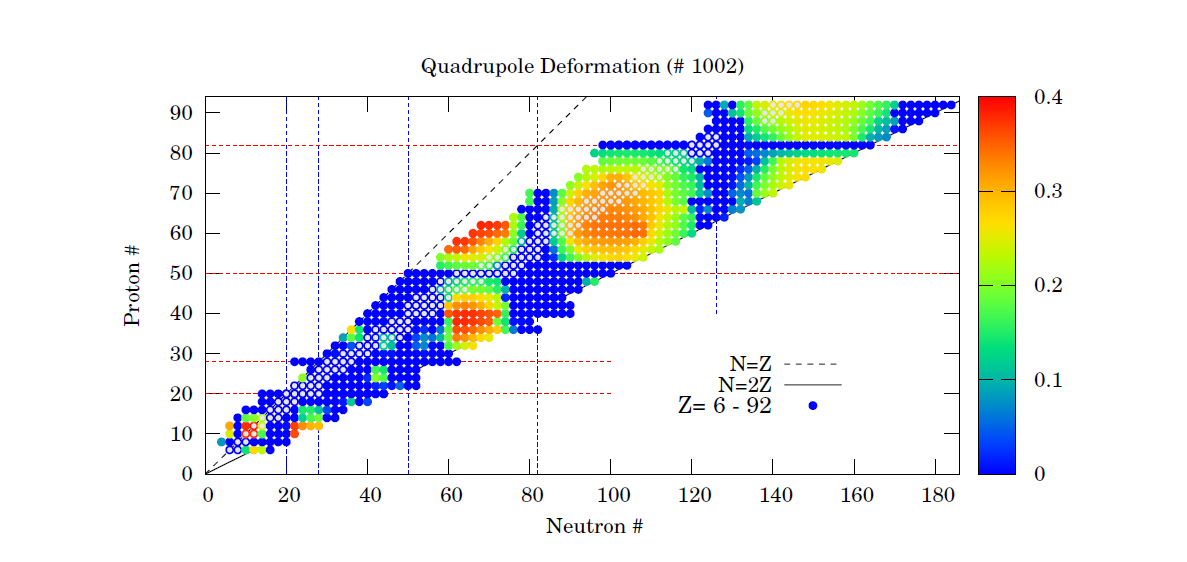
\includegraphics[width=130mm]{../quadrupole_moment_nakatsukasa-san.png}
    \caption{文献\cite{ebata}から引用。変形度$\beta$の絶対値を取ったものに色を付けてプロットしており、赤が濃くなるにしたがって変形が大きいことを表している。
        }\label{fig:deformation_ebata-san}
\end{figure}


%sectionのまとめ
量子多体系である原子核の中では、陽子と中性子を束縛させる強い相互作用と陽子間に働くクーロン相互作用が支配的であるが、本研究ではクーロン相互作用に着目して計算・考察を行った。
過去の研究では斥力であるクーロン相互作用が、原子核の形状や中性子ドリップラインをはじめ様々な物理量にどのような影響を与えるのか報告されたことはなく、本研究は原子核の性質を知る上で重要な役割を果たすことが期待される。
本研究では、クーロン相互作用が原子核の変形度や中性子ドリップラインをはじめとする物理量に与える影響について、系統的な評価をすることを目標とする。

\section{方法}
%本研究では原子核の変形と対相関を自己無撞着に決定することのできる計算プログラムであるHFBTHOを用い、陽子数$Z=2-120$の束縛する偶偶核を対象に数値計算を実行した。
%本研究では化学ポテンシャルを$\lambda_n=\frac{dE}{dN},\lambda_p=\frac{dE}{dZ}$のように設定し、陽子と中性子の化学ポテンシャルが負であることを束縛条件として原子核の存在限界を決定した。
%
エネルギー密度を定義することで他の様々な物理量を計算することのできる密度汎関数理論を用いることで、量子多体系である原子核の性質を探ることが出来る。
本研究ではHFB方程式 (Hartree-Fock-Bogoliubov equation)を解くことのできるHFBTHOプログラムを用いて原子核の様々な性質について調査を行った。
\subsection{HFB方程式}
2体のフェルミ粒子から成る量子系のハミルトニアンは生成・消滅演算子$c,c^\dagger$の組み合わせにより次のように表すことが出来る。
\begin{equation}
    \label{hamiltonian}
    H = \sum_{n_1 n_2} e_{n_1 n_2}c_{n_1}^\dagger c_{n_2} + \frac{1}{4} \sum_{n_1 n_2 n_3 n_4}\bar{v}_{n_1 n_2 n_3 n_4}c_{n_1}^\dagger c_{n_2}^\dagger c_{n_4} c_{n_3},
\end{equation}
ここで$\bar{v}_{n_1 n_2 n_3 n_4}$は反対称性を持つ2体の相互作用の行列要素で、$e$は1体の運動エネルギーである。
HFB法で用いる基底状態の波動関数$\ket{\Phi}$は、準粒子の真空と準粒子の演算子によって$\alpha_k\ket{\Phi} = 0$のように定義される。
ここで準粒子の演算子は元の演算子に対して次のようなBogoliubov変換を行うことで定義される。
\begin{equation}
    \alpha_k = \sum_n(U_{nk}^*c_n + V_{nk}^* c_n^\dagger ),\quad \alpha_k^\dagger  = \sum_n(V_{nk}c_n + U_{nk} c_n^\dagger )
\end{equation}
この変換は次のように書き直すことが出来る。
\begin{equation}
    \left(\begin{array}{c}
            \alpha \\
            \alpha^\dagger
        \end{array}
    \right) =
    \begin{pmatrix}
        U^\dagger& V^\dagger\\
        V^T & U^T
    \end{pmatrix}
    \left(\begin{array}{c}
            c \\
            c^\dagger
        \end{array}
    \right)
\end{equation}
変換のユニタリー性から、行列$U$と行列$V$は以下のような関係を満たしている。
\begin{equation}
    U^\dagger U + V^\dagger V = I, \\
    UU^\dagger  + V^*V^T = I, \\
    U^{T}V + V^{T}U = 0, \\
    UV^\dagger  + V^*U^T = 0. 
\end{equation}
続いて一体の密度行列$\rho$や$\kappa$を次のように定義すると
\begin{equation}
    \label{rho-kappa}
    \rho_{nn'} = \mel{\Phi}{c_{n'}^\dagger c_n}{\Phi} = (V^*V^T){}_{nn'},\quad \kappa_{nn'} = \mel{\Phi}{c_{n'}c_n}{\Phi} = (V^*U^T){}_{nn'}
\end{equation}
ハミルトニアンの期待値を以下のように密度の汎関数として書き換えることが出来る。
\begin{equation}
    \label{func-energy}
    E[\rho,\kappa] = \frac{\mel{\Phi}{H}{\Phi}}{\braket{\Phi}{\Phi}} = {\rm Tr}[(e + \frac{1}{2}\Gamma)\rho] - \frac{1}{2}{\rm Tr}[\Delta\kappa^*]
\end{equation}
ただしここで$\Gamma$と$\Delta$は次のように定義した。
\begin{equation}
    \label{Gamma-Delta}
    \Gamma_{n_1 n_3} = \sum_{n_2 n_4}\bar{v}_{n_1 n_2 n_3 n_4}\rho_{n_4 n_2},\quad \Delta_{n_1 n_2} = \frac{1}{2}\sum_{n_3 n_4}\bar{v}_{n_1 n_2 n_3 n_4}\kappa_{n_3 n_4}
\end{equation}
ここで式\eqref{func-energy}の変分を取ることで最終的に、次の形をしたHFB方程式を得る。
\begin{equation}
    \label{HFBequation}
    \begin{pmatrix}
        e + \Gamma - \lambda & \Delta \\
        - \Delta^* & - (e + \Gamma){}^* + \lambda
    \end{pmatrix}
    \left(
        \begin{array}{c}
            U \\
            V
        \end{array}
    \right) =
    E
    \left({}
        \begin{array}{c}
            U \\
            V
        \end{array}
    \right)
\end{equation}
式\eqref{HFBequation}での$\lambda$はラグランジュの未定乗数であり、正しい粒子数を補正するために導入されている。
この化学ポテンシャルは陽子と中性子それぞれにおいて$\lambda_p=\frac{dE}{dZ}, \lambda_n=\frac{dE}{dN}$であり、本研究ではこれらが負であることを束縛条件として原子核の存在限界を決定した。
HFBTHOプログラムでは式\eqref{rho-kappa}から式\eqref{HFBequation}を、$n$回目の試行で得られた式\eqref{HFBequation}の固有値$E$と
$n+1$回目の試行で得られた式\eqref{HFBequation}の行列要素の全てが限りなく同じ値になるまで繰り返し解く。
最後の試行で得られた密度行列$\rho$やペアリング行列$\kappa$を用いて様々な物理量を定義し、原子核の性質を詳しく調べた。

\subsection{四重極演算子}
\begin{equation}
    \label{quadrupole-moment-func}
    \hat{Q}_{20}(r,\theta,\phi) = r^2 \sqrt{\frac{5}{4\pi}} P_2(\cos{\theta})
\end{equation}
$P_2$は2次のラグランジュ多項式である。

\subsection{変形度$\beta$}
四重極演算子の期待値から四重極モーメントが得られる。
得られた四重極モーメントと対応した原子核の変形度を表すことが出来る指標に変形度がある。
本研究では$\beta$と表記する。定義は次のとおりである。
\begin{equation}
    \label{beta-func}
    \hat{Q} = \sqrt{\frac{5}{\pi}}\ev*{r^2}\hat{\beta}
\end{equation}
\begin{equation}
    \langle \hat{Q}_{20}\rangle = \int d\boldsymbol{r} Q_{20}(r,\theta,\phi) \rho(r,\theta,\phi),
\end{equation}
\begin{equation}
    \langle r^2 \rangle = \int d\boldsymbol{r}  r^2 \rho(r,\theta,\phi),
\end{equation}

\subsection{ペアリングギャップ}
\subsection{半径}
\subsection{1粒子準位}

\subsection{計算のセッティング}
本研究に用いたHFBTHOプログラム内の諸設定については以下のように行った。
・模型空間:$N=20$
・核力の相互作用項:Skyrm型の相互作用、SLy4とSkM*
・ペアリングエネルギー:SLy4で-287MeV,SKM*で-240MeV
さらにクーロン相互作用を調べるために関連する相互作用にも変化を加えて計算を行った。
2種類の相互作用の双方においてdirect termとexchange termの2種類を切ったものと、入れたものを比較した。
表に示した方が良い。
さらに変形について調べるために$Z=44-54,N=40-58$の核に対しては変形度を固定した計算を実行することで、エネルギーを変形度の関数として調べた。

\section{結果}
陽子数$Z=2$から$Z=120$の偶偶核についてSLy4型の汎関数とSKM*型の汎関数で計算を実行した。
SLy4型の計算を実行したものの内、核子の化学ポテンシャルがともに負の原子核の変形度$\beta$を 図\ref{fig:SLY4_ON}にプロットした。
変形度$\beta$は軸対称の変形を示しており、プロレート型の変形とオブレート型の変形の区別はせず、大きく変形している原子核を赤色で示している。
図\ref{fig:SLY4_OFF}はクーロン相互作用を外した場合の計算結果である。
\begin{figure}[ht]
    \centering
    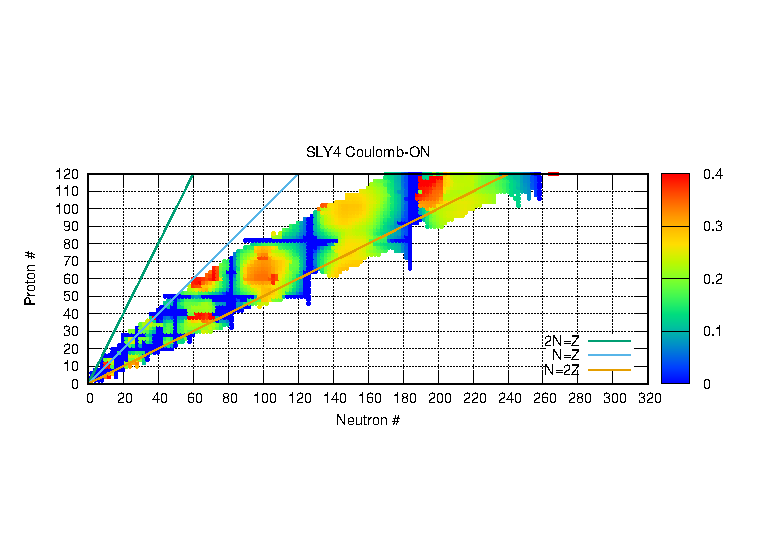
\includegraphics{../SLY4_ON.eps}
    \caption{SLy4汎関数を用いた計算におけるクーロン相互作用を入れた場合の原子核の変形度$\beta$}\label{fig:SLY4_ON}
\end{figure}
\begin{figure}[H]
    \centering
    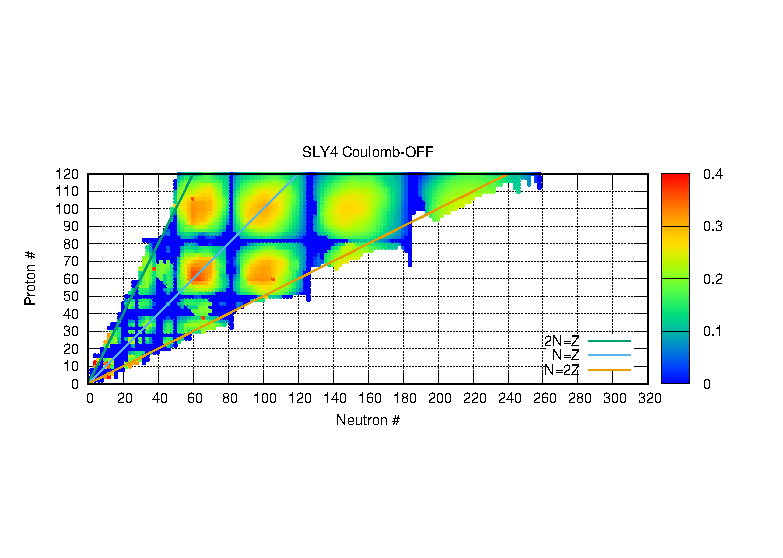
\includegraphics{../SLY4_OFF.eps}
    \caption{SLy4汎関数を用いた計算におけるクーロン相互作用を入れない場合の原子核の変形度$\beta$}\label{fig:SLY4_OFF}
\end{figure}
続いてSKM*型の汎関数による計算結果を図○○から図○○に示す。
%subsectionで分ける必要はない?
%核図表から見て取れる内容ここから

\subsection{陽子ドリップラインの変化}
図\ref{fig:SLY4_ON}と図\ref{fig:SLY4_OFF}を比べた際にいちばんに目に付くのは、クーロン相互作用がない仮想的な状況では陽子のドリップラインが陽子過剰側に大きくシフトする点である。\ref{fig:SLY4_OFF}陽子間に働くクーロン力が0になり、今回用いたエネルギー密度汎関数はアイソスピン対称性を持つため、$N=Z$の線に対して対称である。
今回の研究では陽子数$Z=2-120$の偶偶核のみを対象に計算を実行したため$Z \le 120$の範囲でしか陽子と中性子の対称性は再現できていないが、より大きな陽子数であっても同様の結果が得られる。
またクーロン相互作用がない場合には斥力が消え核力のみに束縛されることになるため、いくらでも大きな原子核が存在する。

\subsection{魔法数の原子核}
続いて図\ref{fig:SLY4_ON}において陽子または中性子が魔法数の原子核では変形が小さくなると同時に、魔法数に近づくにつれて変形度は小さくなり、魔法数を超えて再び大きくなるような挙動が確認できる。
この現象は特に中性子では50以降、陽子では28以降の魔法数において始まり、核子数が大きくなるにしたがって顕著である。
また核子が魔法数の原子核では束縛される原子核が増えることも分かる。
魔法数より小さな核子数の時には束縛されていなかったような核子であっても、殻効果の影響で原子核がエネルギー的に安定することで魔法数では再度束縛される。
そして再び魔法数を超え束縛が解かれることでドリップラインを迎える。
原子核は核子が魔法数に近づくにつれて変形が小さくなり、束縛状態の核が増えるという予測に基づくと$Z=258$付近にも未だに一般に知られていない魔法数が存在していることが予測される。
また陽子数$Z=10-18$の同位体では$N=28$付近であっても変形するような原子核が存在する。
そのほかにも、中性子が魔法数の同調体に着目した際には陽子数にかかわらずにほとんどの原子核で球形であるのに対し、
陽子数が魔法数の同位体では特定の中性子数で変形して存在することが確認でき、こちらも興味深い結果である。
クーロン相互作用のない図\ref{fig:SLY4_OFF}であっても$Z=82$の同位体では$N=150-172$で、
$Z=50$の同位体では$N=98-110$、$Z=28$の同位体では$N=12-18$の領域で変形している。

\subsection{中性子過剰な原子核について}
同種粒子の間に働く核力よりも異種核子同士の間に働く核力の方が強い性質がある。
また陽子や中性子はフェルミ粒子であるため、パウリの排他律から同じ状態には1つの粒子しか入れない。
質量数が同じ原子核でエネルギーの最も低い状態から順番に粒子を入れていったときには、同種粒子を多く入れた状態よりも異種粒子と数を合わせた状態の方が、原子核のエネルギーとしては安定する。
以上2つの性質のみを考えると原子核は核子数が$N=Z$であるような状態でいちばん安定すると考えられる。
しかし実際には陽子間にクーロン相互作用による斥力が働いているため、陽子数が大きくなるような原子核では中性子過剰の方が安定して存在する。
図\ref{fig:SLY4_ON}では実際に、陽子数$Z=62$以降の原子核では$N=Z$で束縛するような原子核は存在せず、陽子数が増えていくにつれて中性子過剰で安定するような原子核が増えていく。
%核図表から見て取れる内容ここまで

%変形度の話ここから
\subsection{変形度の増大}
図\ref{fig:SLY4_ON}と図\ref{fig:SLY4_OFF}を比較することでクーロン相互作用が原子核に与える影響を評価する。
変形度に着目すると核図表全体に渡って増加傾向にある。
一例として$Z=46,N=48$と$Z=52,N=54$の原子核におけるエネルギーを変形度の関数として調べた。
この計算は変形度に拘束条件を与えたまま実行し、任意の変形度におけるエネルギー最小値を求めた。
図\ref{fig:ene_beta_52-54}には$Z=52,N=54$の結果を、図\ref{fig:ene_beta_46-48}には$Z=46,N=48$の結果を示す。
横軸に変形度$\beta$を指定し、原子核の基底状態での変形度がクーロン相互作用によって変化することを確認した。
縦軸にはエネルギーを表示しているが、変形度が$\beta=0$のエネルギーが0となるように設定した。
\begin{figure}[ht]
    \centering
    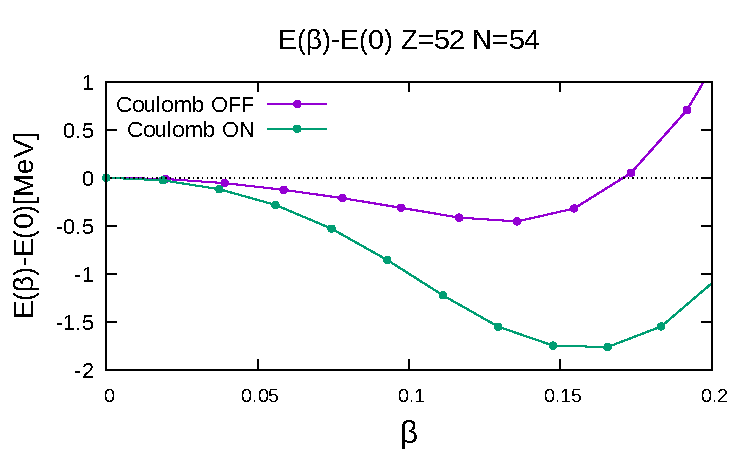
\includegraphics{../Z=52_N=54_energy_beta.pdf}
    \caption{
        $Z=46,N=48$におけるSLy4汎関数を用いた計算による変形度$\beta$に対する原子核のエネルギー
        }\label{fig:ene_beta_52-54}
\end{figure}
\begin{figure}[ht]
    \centering
    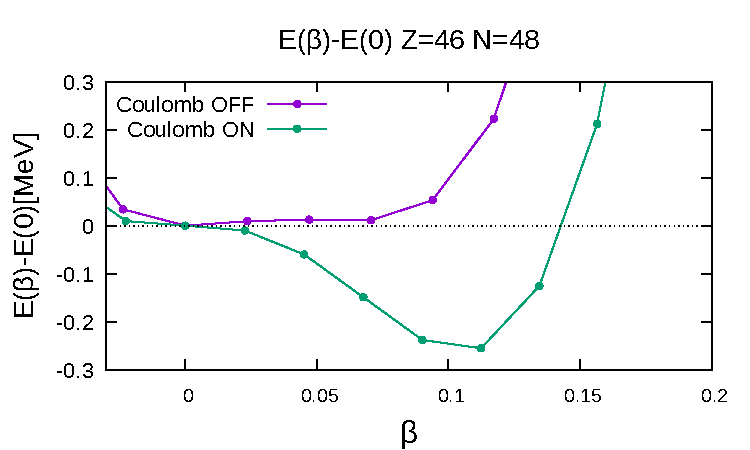
\includegraphics{../Z=46_N=48_energy_beta.pdf}
    \caption{
        $Z=46,N=48$におけるSLy4汎関数を用いた計算による変形度$\beta$に対する原子核のエネルギー
        }\label{fig:ene_beta_46-48}
\end{figure}
図\ref{fig:ene_beta_52-54}からは、クーロン相互作用によって基底状態の変形度が増加していることが分かる。
またクーロン相互作用がある時の方が、基底状態のエネルギーと変形していないときのエネルギーの差が大きくなっている。
続いて図\ref{fig:ene_beta_46-48}では、クーロン相互作用がないときには球形として存在していたものが、クーロン相互作用を入れることによって変形して存在するようになる。
クーロン相互作用のエネルギーは原子核半径の逆数に比例して減少していくことから、原子核を変形させて陽子同士の距離を広げることでエネルギー的に安定させる方向に作用していることが予想される。
%変形度の話ここまで

%ドリップラインの話ここから
\subsection{中性子ドリップラインの拡大}
図\ref{fig:SLY4_ON}と図\ref{fig:SLY4_OFF}から、クーロン相互作用によって陽子ドリップライン、中性子ドリップラインに変化が現れることが分かった。
陽子ドリップラインはクーロン相互作用によって大きく右側にシフトするが、これは古典的にも直感的にも想像し易い結果である。
陽子間に働く斥力の影響で原子核が不安定化するため、陽子数に比べて中性子数が多いような状態を取ることで原子核全体としては安定する傾向にある。
一方クーロン相互作用によって中性子ドリップラインも中性子過剰側にシフトしている。
斥力のクーロン相互作用の効果で束縛される原子核が増加するというのは、直感的にも古典的にも理解することが難しい結果である。
\begin{figure}[H]
    \centering
    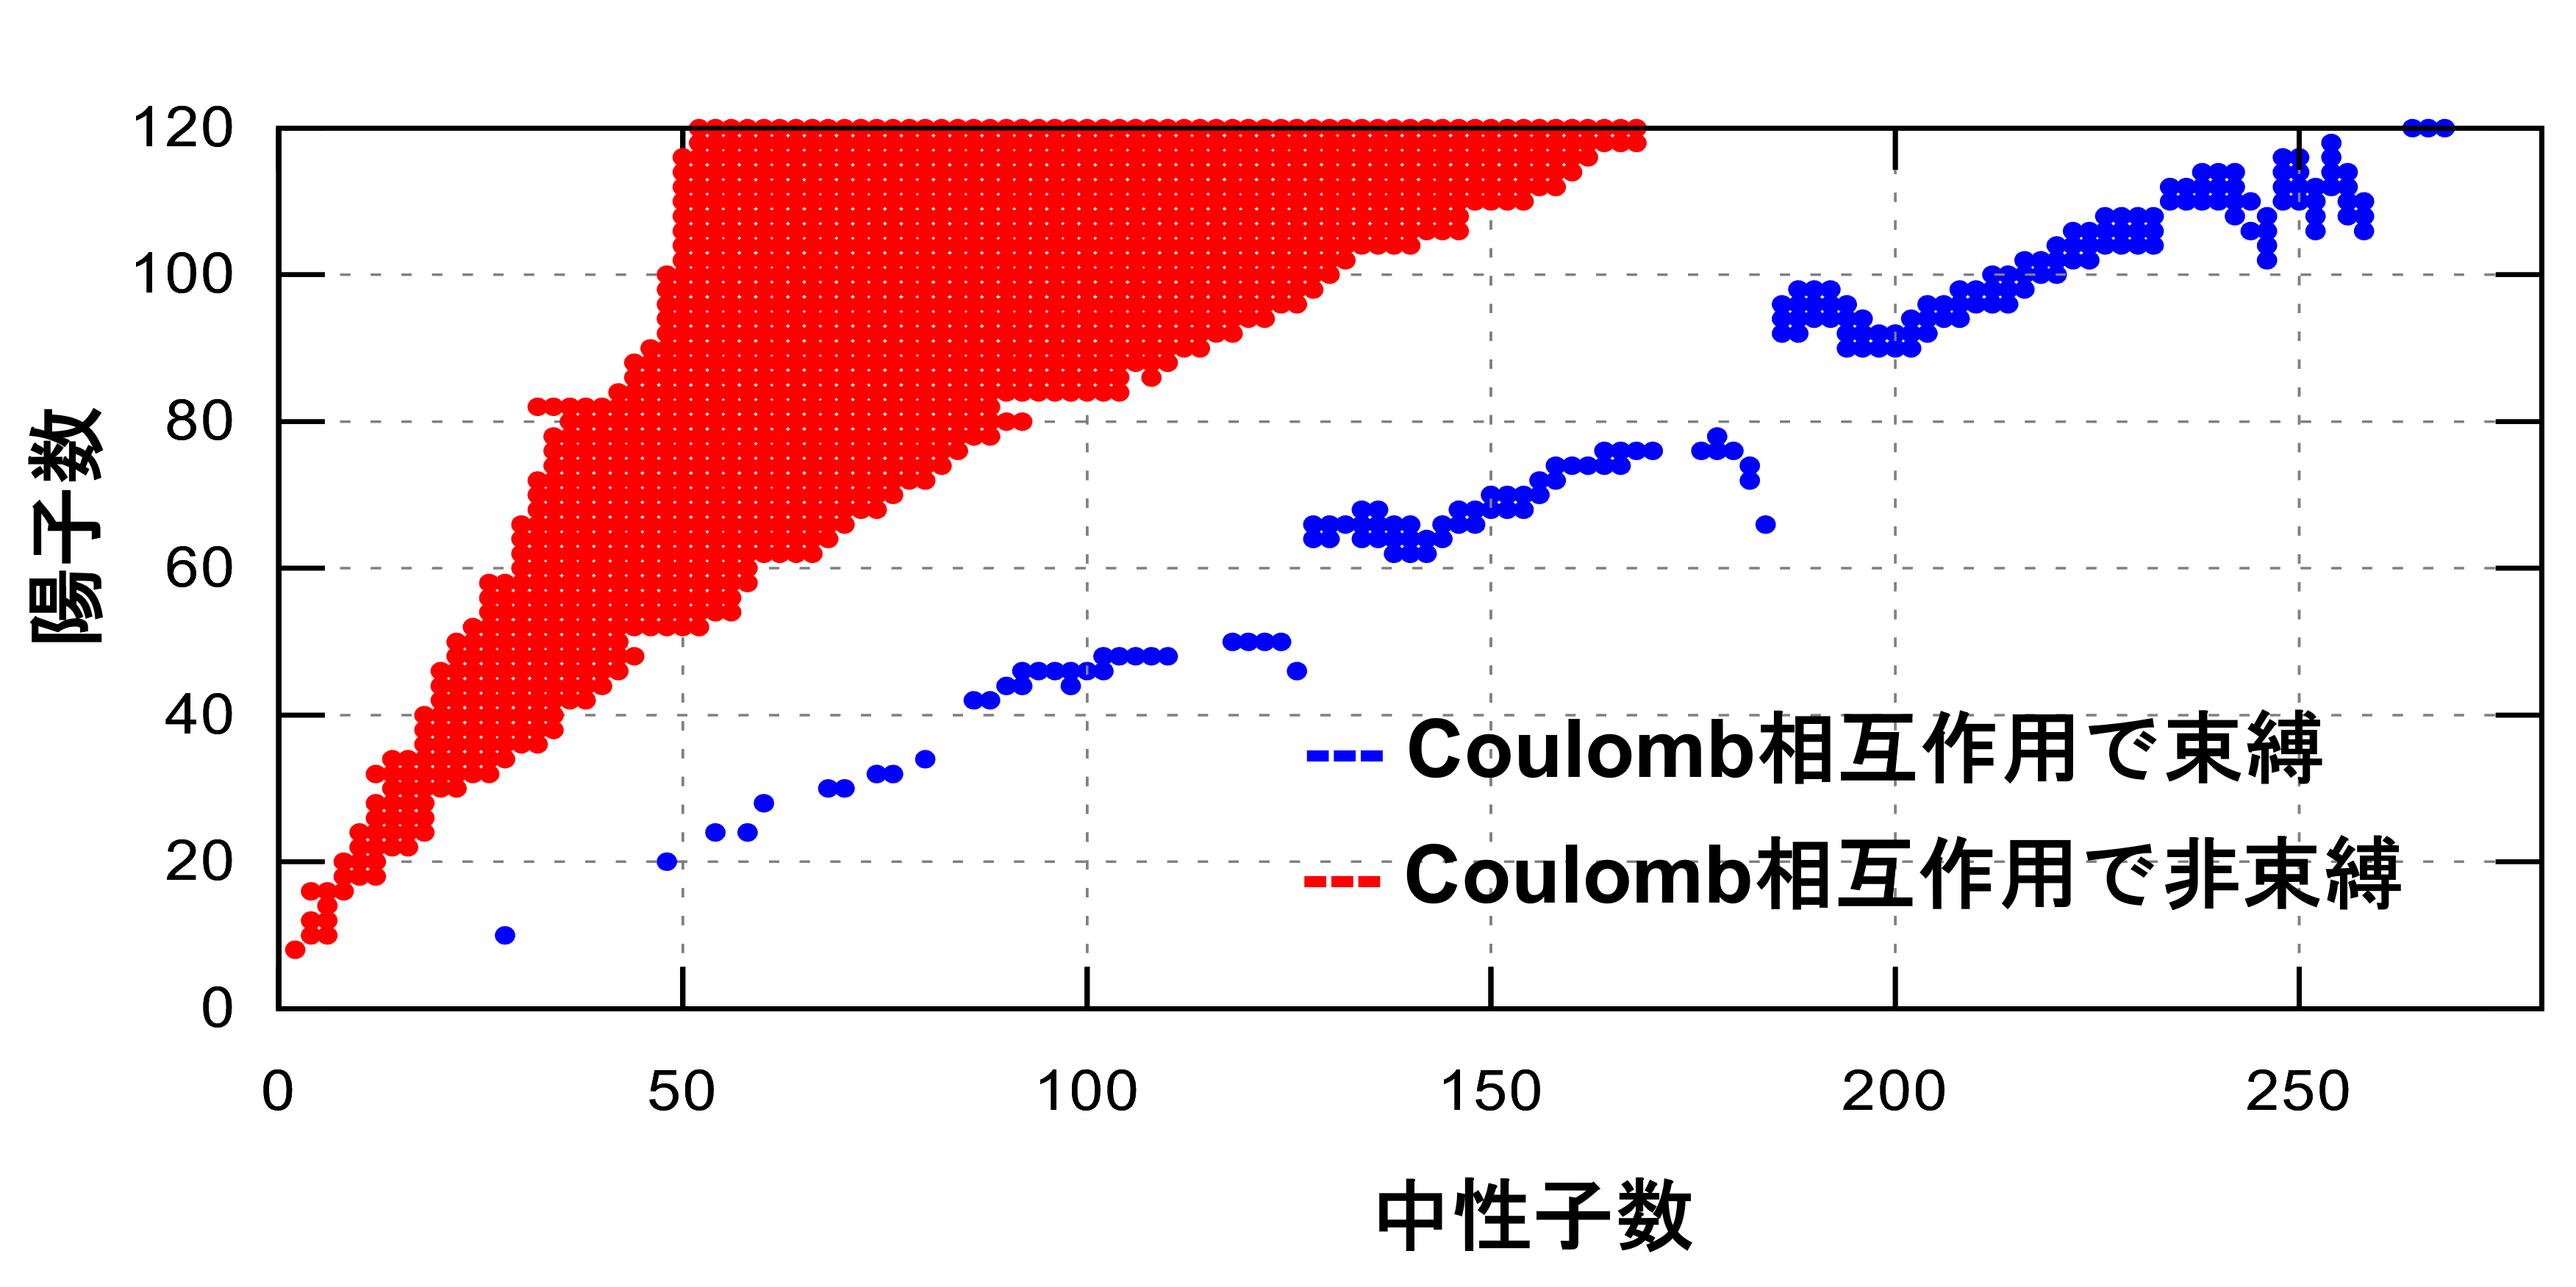
\includegraphics[width=130mm]{../ドリップラインの変化.png}
    \caption{
        クーロン相互作用により束縛が解けた原子核を赤色に、新たに束縛するようになった原子核を青色で表している。
    }\label{fig:ドリップラインの変化}
\end{figure}
図\ref{fig:ドリップラインの変化}にはクーロン相互作用によって束縛の有無が変化する原子核を示した。
赤色は束縛が解ける原子核で、青色が新たに束縛される原子核である。
つまり陽子ドリップラインの変化を赤色で、中性子ドリップラインの変化を青色で示している。
特に中性子ドリップラインがより中性子側にシフトするという結果は大変興味深く、図\ref{fig:SLY4_ON}と対応させながら確認すると、変形状態で束縛される原子核のみならず、球形状態で新たに束縛される原子核も存在することが分かった。
これまでの研究で原子核が変形することによりエネルギー的に安定となることは指摘されているが、球形のままエネルギー的に新たに束縛されるような原子核が存在することも大変興味深い。
変形の効果を考慮せずにクーロン相互作用の影響を評価するため球形のままドリップラインを拡大させている原子核に着目し、$Z=50,N=116,120$の一粒子準位を調べたところ、エネルギーに変化が現れることが確認された。
結果を図\ref{fig:spe50-116}、図\ref{fig:spe50-120}に示す。
\begin{figure}[H]
    \centering
    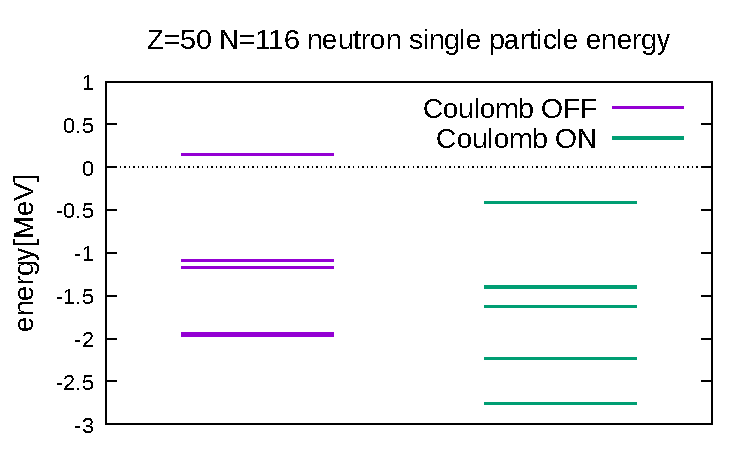
\includegraphics{../Z=50_N=116_speN.pdf}
    \setlength\floatsep{0pt}
    \caption{
        $Z=50,N=116$の中性子の一粒子準位のクーロン相互作用の有無による比較
        }\label{fig:spe50-116}
\end{figure}
\begin{figure}[H]
    \centering
    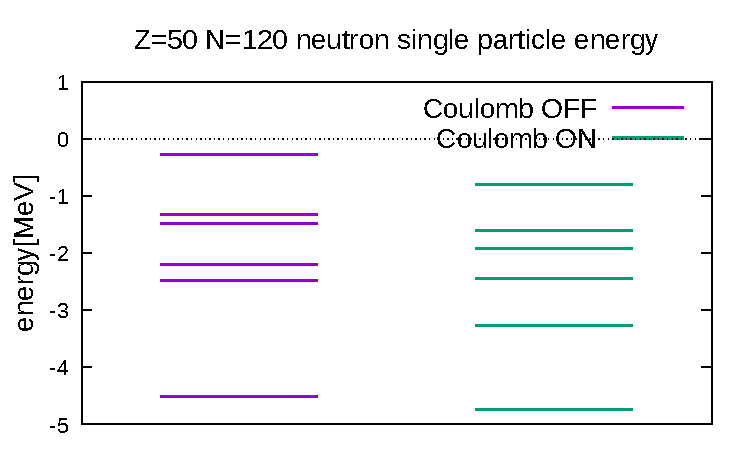
\includegraphics{../Z=50_N=120_speN.pdf}
    \setlength\floatsep{0pt}
    \caption{
        $Z=50,N=120$の中性子の一粒子準位のクーロン相互作用の有無による比較
        }\label{fig:spe50-120}
\end{figure}
図\ref{fig:spe50-116}、および図\ref{fig:spe50-120}から0 MeV付近ではクーロン相互作用によって中性子の一粒子エネルギーが減少し、結果として化学ポテンシャルも減少することが分かった。
クーロン相互作用による中性子ドリップラインの中性子過剰側へのシフトは、このようなメカニズムによって引き起こされると結論付けられる。
%ドリップラインの話ここまで
%
%半径の話ここから
%このサブセクションは中性子の一粒子準位がなぜ変化するのかを考察する内容
%\subsection{半径の増加}
%またクーロン相互作用と原子核の半径にも相関があることを確認した。
%図\ref{fig:multi_SLY4_beta_radius_Z=50.eps}~図\ref{fig:multi_SLY4_beta_radius_Z=90.eps}では$Z=50$と$Z=90$の変形度$\beta$と半径を、中性子数の関数として表示した。
%これらの図では核子の化学ポテンシャルは考慮せず、計算を実行したものを全てプロットした。
%この結果からクーロン相互作用により変形の有無に依らずに原子核の半径が増加することが分かった。
%これは斥力により陽子同士の間隔が広がり、それに呼応する形で原子核全体の半径が増加するようなメカニズムであると予想される。
%また中性子のドリップライン内では有意な差として確認できるが、ドリップライン外側の中性子過剰核ではクーロン相互作用の有無に依る差が小さくなっていることも分かる。
%これは陽子数に対して中性子の数が多くなることで、クーロン相互作用の効果が弱まることが要因であると考えられる。
%\begin{figure}[H]
%    \centering
%    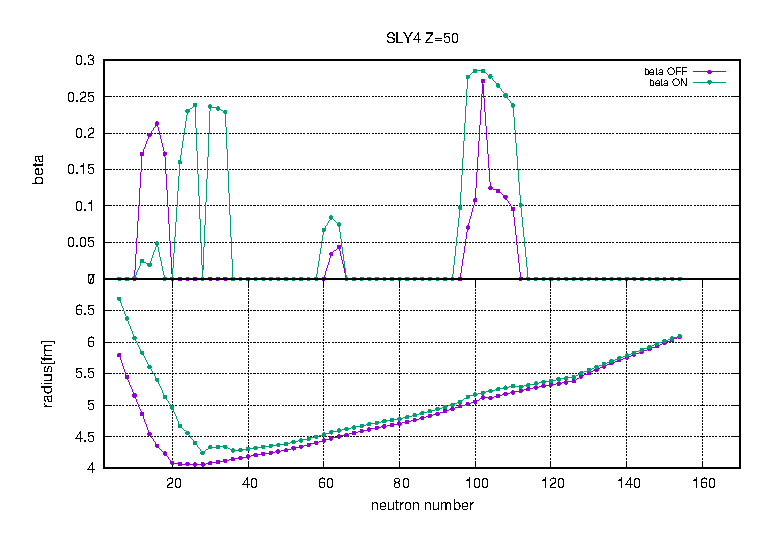
\includegraphics{../multi_SLY4_beta_radius_Z=50.eps}
%    \setlength\floatsep{0pt}
%    \caption{$Z=50$の変形度と半径}\label{fig:multi_SLY4_beta_radius_Z=50.eps}
%\end{figure}
%\begin{figure}[H]
%    \centering
%    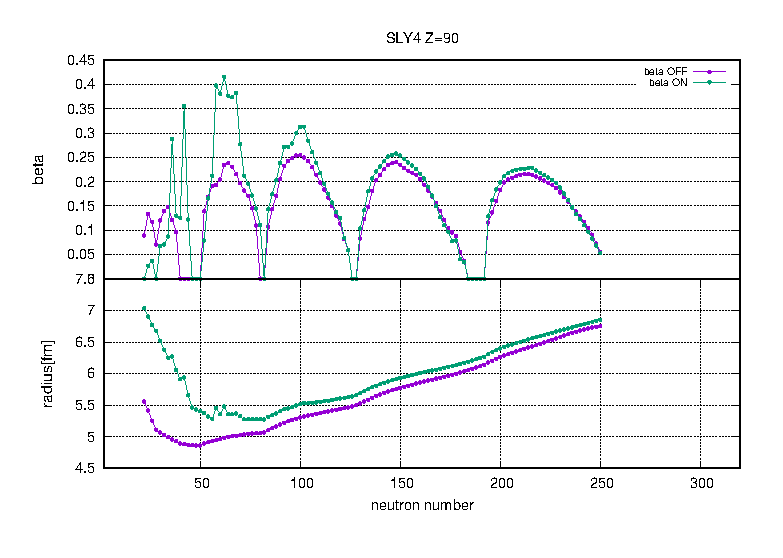
\includegraphics{../multi_SLY4_beta_radius_Z=90.eps}
%    \setlength\floatsep{0pt}
%    \caption{$Z=90$の変形度と半径}\label{fig:multi_SLY4_beta_radius_Z=90.eps}
%\end{figure}
%半径の話ここまで

\section{結論}
HFBTHOプログラムを用いた系統的な計算から、クーロン相互作用によって原子核の変形度は増加し、中性子ドリップラインは拡大する。
斥力により原子核の半径が増加することから核子の1粒子エネルギーが変化し、$0[MeV]$付近では一粒子準位が下がる。
その結果により中性子の化学ポテンシャルが減少することで中性子ドリップラインが拡大する。
また図\ref{fig:ene_beta_52-54}と図\ref{fig:ene_beta_46-48}からクーロン相互作用が原子核の変形度を増加させることも示された。

\section{展望}
本研究ではクーロン相互作用に着目して変形度や中性子ドリップラインについて議論した。
特に中性子ドリップラインに関しては球形核の一粒子準位が変化することから中性子過剰側により多くの原子核が存在する結果を得た。
今後はクーロン相互作用の影響だけでなく、変形度を固定した状態での一粒子準位を調べることで、変形が中性子ドリップラインにどのような影響を及ぼすのかを評価したい。
また今回の研究では四重極変形にのみ着目し、さらにプロレート変形とオブレート変形の違いは考慮しなかった。
プロレート変形とオブレート変形の違いが原子核に対してどのように作用するのか評価することも、今後の研究において解明されることが期待される。

\begin{thebibliography}{99}
\bibitem{hfbtho1}
M. V. Stoitsov, J. Dobaczewski, W. Nazarewicz, and P. Ring,
%Axially deformed solution of the Skyrme-Hartree-Fock-Bogolyubov
%equations using the transformed harmonic oscillator basis: The Program
%HFBTHO (v1.66p),
Comput. Phys. Commun. \textbf{167}, 43 (2005).
\bibitem{hfbtho2}
M.V. Stoitsov, N. Schunck, M. Kortelainen, N. Michel, H. Nam, E. Olsen,
J. Sarich, and S. Wild,
%Axially deformed solution of the Skyrme-Hartree-Fock-Bogoliubov
%equations using the transformed harmonic oscillator basis (II) hfbtho
%v2.00d: A new version of the program,
Computer Physics Communications \textbf{184}, 1592 (2013).
\bibitem{ebata} S. Ebata and T. Nakatsukasa, Phys. Scr. \textbf{92},
064005 (2017).
\bibitem{RingSchuck}
P. Ring and P. Schuck, \emph{The Nuclear Many-Body Problem}
(Springer-Verlag, 1980).
\bibitem{NuclearStructure}
S. G. Nilsson and I. Ragnarsson,
\emph{Shapes and Shells in Nuclear Structure}
(Cambridge University Press, 1995).
\end{thebibliography}
\end{document}